\section{Field Programmable Gate Array (FPGA)} \label{sec:fpga}
%
%
As developed in the Introduction, the focus on this study is on accelerating the inference stage on \acrshort{fpga}. According to \textcite{mittal_survey_2015}, \acrshort{fpga}s provide higher energy efficiency than both \acrshort{gpu}s and \acrshort{cpu} and higher performance than \acrshort{cpu}s. Besides, \acrshort{fpga}s are very flexible hardware that can be tailored for each particular \acrshort{nn} \cite{vestias_fast_2019}. Furthermore, we can expect in the future that \acrshort{fpga}s will provide higher performance for performing \acrshort{cnn}s to \acrshort{gpu} \cite{nurvitadhi_can_2017}.

According to \textcite{harris_digital_2015}, the definition of an \acrshort{fpga} is: \textquote{\textit{a \acrfull{fpga} is an array of reconfigurable gates}}. The characteristic of this platform is that it can implement combinational and sequential logic but also multilevel functions. An \acrshort{fpga} also integrates built-in multipliers, high-speed I/Os, data converters, large RAM arrays, and processors.

An illustration of the general \acrshort{fpga} layout is provided in Figure \ref{fig:fpga}. An \acrshort{fpga} consists of an array of configurable logic elements (LE), also called configurable logic blocks (CLB) \cite{harris_digital_2015}. Each \acrshort{le} can be configured to execute either combinational or sequential logic. Each \acrshort{le} is connected to other \acrshort{le}s to form an array. To interface with the outside world, the array is connected to a set of \acrfull{ioe}.
%
\begin{figure}[H]
    \centering
    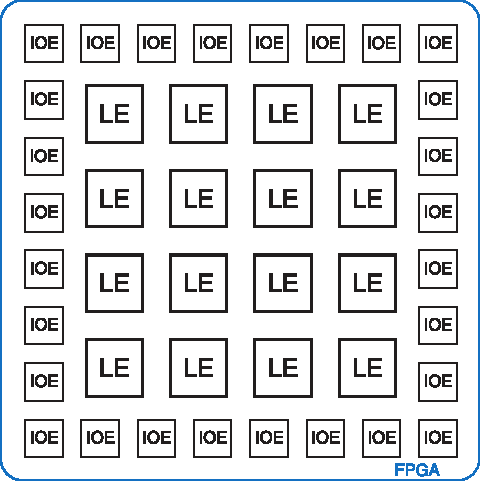
\includegraphics[width=0.4\textwidth]{fpga.pdf}
    \caption{General \acrshort{fpga} layout, from \cite{harris_digital_2015}}
    \label{fig:fpga}
\end{figure}

Designs can be implemented on an \acrshort{fpga} using a software programming tool that can use either a \acrfull{hdl} or a schematic. An \acrshort{hdl} is a language that gives the specifications of digital design. The interest of using this language is the fast development cycle compared to a schematic, due to the higher abstraction level and the gate optimizations \cite{harris_digital_2015}. The most popular \acrshort{hdl} are \textit{VHDL} and \textit{SystemVerilog} which mostly differ on syntax. The architecture of this work is implemented in \textit{SystemVerilog}. 

The design flow of an \acrshort{fpga} can be described as follows \cite{barte_value-added_2011}. First, the programmer creates the design of interest using either a schematic or \acrshort{hdl}. Second, the design is synthesized, which means that the software determines how to configure the components of the \acrshort{fpga} to execute the specified function. Third, the software assesses if the design is correct using a functional simulation. If it is correct, the software fits the element into the \acrshort{fpga} and does the \textbf{timing analysis}. This step simulates the real delay to check if the timing requirements are met. Finally, the design is programmed into the \acrshort{fpga} when the timing analysis simulation is correct.

To perform a functional simulation of the proposed \acrfull{dut}, we can use a \textit{testbench} \cite{harris_digital_2015}. According to \textcite{harris_digital_2015},\textquote{\textit{The testbench contains statements to apply inputs to the \acrshort{dut} and ideally, to check that the correct outputs are produced}}. However, this practice is tedious and error-prone. Instead, we can use a \textit{self-checking testbench}. In the frame of this thesis, we chose an alternative approach. Since we have to verify a huge number of outputs, instead the testbench produces an \textit{output file}, which contains all outputs produced by the \acrshort{dut}. Therefore, we can compare the obtained results with the expected ones using a programming language (\textit{Python} has been used).